\chapter{Machine Learning, a field of AI}\label{chap:chap3}

\section*{}

\paragraph{}Machine Learning is a subfield of Artificial Intelligence (AI), a branch of computer science whose  fundamental aim is to develop computational systems (smart machines) that show operational behaviour and are capable of performing tasks that typically require human intelligence \citet{Spalding1981}. Those algorithms often exceed the capabilities of human at doing thise tasks.

\begin{figure}[ht]
    \centering
    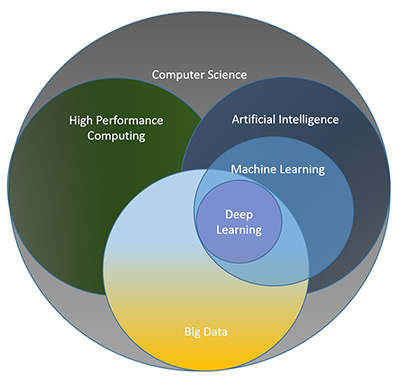
\includegraphics[scale=0.6]{figures/ai.jpg}\citet{ai}
    \caption{Machine learning and directly related areas}
    \label{fig:ML}
\end{figure}

\section{Historical Perspective}
\paragraph{}The field of AI began in the 1940s with Alan Turing, an  English mathematician and computer scientist. Who is widely know as the father of Artificial Intelligence and Computer Science \citet{beavers2013alan}.
His outstanding achievements include: 
\begin{itemize}
\item  Cracking the Enigma code which,  according to Keegan, was allegedly decisive in the course of the Second World War. As a result the war was significantly shortened and cracking the Enigma code contributed to the known outcome \citet{Keegan2003}. 
\item Inventing of the first model for the general-purpose computers: Turing machine \cite{Booker_turingand}
\item Creating the Turing test, currently used, to find out whether an intelligent agent is capable of thinking like a human being. Through a conversation in natural language between a human and a computer, a human evaluator has to try to distinguish the computer from the human. When this happens, the test is negative. Else, it means that a computational system achieves a human-like level of artificial intelligence \citet{Bowen2016}.
\end{itemize}\espaco

Up to this moment applications have been developed in the Narrow AI branch, this means that AI tries to perform well on one task, rather than strive for human intelligence, named Artificial General Intelligence (AGI) or beyond the best human brains of that, named Artificial Super Intelligence (ASI).

\iffalse
\begin{figure}[ht]
    \centering
    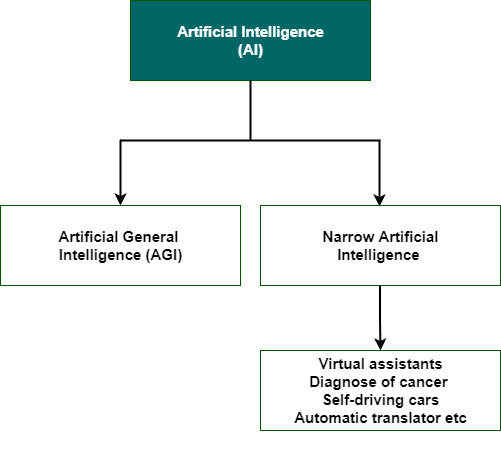
\includegraphics[scale=0.6]{figures/AIBranchs.png}
    \caption{Types of AI}
    \label{fig:AIt}
\end{figure}
\fi

\begin{figure}[ht]
    \centering
    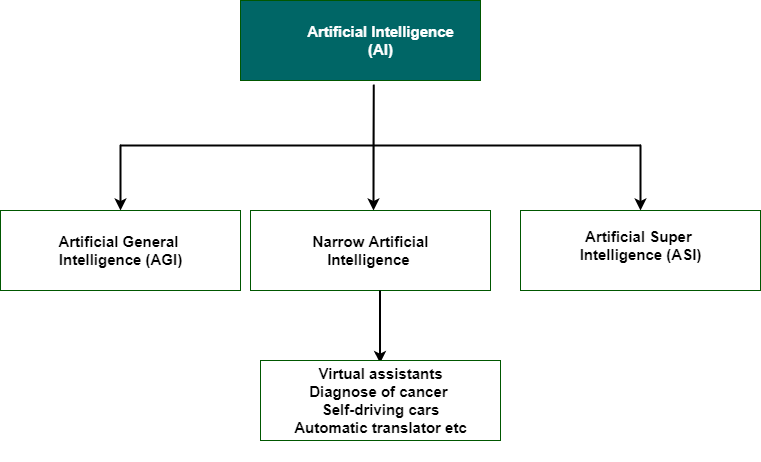
\includegraphics[scale=0.6]{figures/AItypes.png}
    \caption{Types of AI}
    \label{fig:AIty}
\end{figure}




To reach the same objectives that make people seem intelligent, behind the study of those processes/principles that make computers execute tasks similar to those of humans in stereotyped situations and  more effectively  \citet{russell2016artificial}.  
Programming techniques, like nondeterministic search, are based, at least partially, on declarative languages, namely logic-based, functional or object-oriented.


\subsection{The evolution of AI in board games}


\paragraph{} The theory of neural network (NN) began in 1943 using electrical circuits as a nerve cell with a logic gate with binary outputs.  In the 1950s, computer scientists simulated the idea in their work, a hypothetical NN.


Over time, we have seen successive application of artificial intelligence in board games, because they are both understandable and complex.

Followed events chronologically:
\begin{itemize}
    \item  In the 50's, the investigation on the game of checkers stands out.
    So learn by playing and giving a set of rules game as well a sense of direction and some parameters without including the weight of your importance.
    Arthur Samuel developed software that helped the IBM computer get better at checkers,  the more it played.
    With the premise of the possibility of scaling and transposing these machine learning techniques to other areas \cite{Samuel}.
    \item Already in 1997, IBM's Deep Blue (chess-playing computer), capable of evaluating 200 million positions per second (twice as fast as the 1996 version), beat grandmaster Garry Kasparov.
    \item And more recently in 2016, human intelligence head to head with machines, AlphaGo — AI program powered by Google. The game Go, is considered the oldest in the world and probably the most complex. Google DeepMinds AlphaGo combines reinforcement learning techniques with simulation so is powered with all types of Go matches, and then study, learn from them, and discover your own moves. It knows the rules, and discovers highly efficient creative moves never before thought of by humans \citet{Silver2017} .
    
    
\end{itemize}

\espaco
Due to the evolution of the processing power of computers, it is now possible to run computationally demanding algorithms in terms of calculations and/or the amount of data used \citet{history}.
In this way, there was a path that made possible a new era, a revolution
of Artificial intelligence
called deep learning,
that mimics neural networks
of the human brain.

\newpage
\subsection{Perceptron}

\paragraph{}The Perceptron is like an atom of artificial intelligence that performs computations to extract information or knowledge from input data \cite{Rosenblatt}.

\begin{figure}[ht]
    \centering
    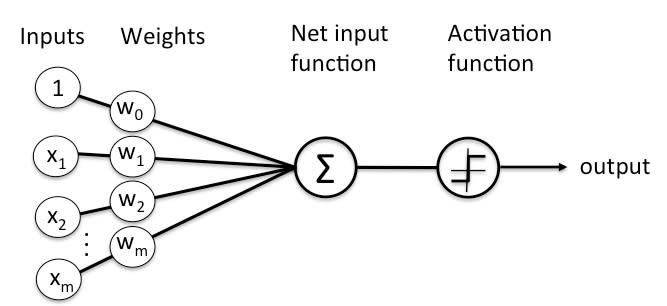
\includegraphics[scale=0.6]{figures/general-diagram-of-perceptron-for-supervised-learning_4.jpg}
    \caption{Perceptron model representation}
    \label{fig:PercMR}
    \citet{perc}
\end{figure}




\section{Machine Learning types}
Machine learning algorithms are
categorized into three main categories:
\begin{itemize}
\item supervised learning \ref{SL}
\item unsupervised learning
\item reinforcement learning
\end{itemize}

\subsubsection{Supervised learning}\label{SL}

\paragraph{}The process of creating the machine learning model involves having a dataset that contains the features and labels in order to use it to classify any given new point of data \citet{Burkov2020}.

Within supervised learning we can divide into: 
\begin{itemize}
    \item  Classification performing as a category the class or label (y)
    \item Regression if we consider as a class(y) a continuous variable
\end{itemize}   
 Examples: 
 
 \textbf{Linear Regression}, assumption: the class is expected to be a linear combination \ref{LRform} of the features!  It could be adapted for higher dimensions.  
 
 $f(X)=\beta_{0}+\beta_{1}X_{1}+\beta{2}X_{2}+...+\beta_{p}X_{p}$ \label{LRform}
 
 \espaco
 

There are two types of algorithms:
\begin{itemize}
    \item \textbf{Lazy} like:
\begin{itemize}
\item  K-Nearest Neighbours or KNN  (distance based technique)

When a new point appears, we calculate the similarity (or distances, as in clustering) of the K-nearest Neighbours. Where k is a positive number, to obtain optimal value should use an error plot or accuracy plot.
The class of our new input is assigned to the class most common, like voting system in democracy \citet{MULLER2019145}.

\item Rule Based


A technique widely used in healthcare in the 70s. However, it has its limitations in comparison with the techniques used today. Those limitations include high monetary cost, dependence on specialized human resources, and complexity of how to update the rules. Practical implementation constraints are illustrated in the table below. 


\begin{figure}[ht]
    \centering
    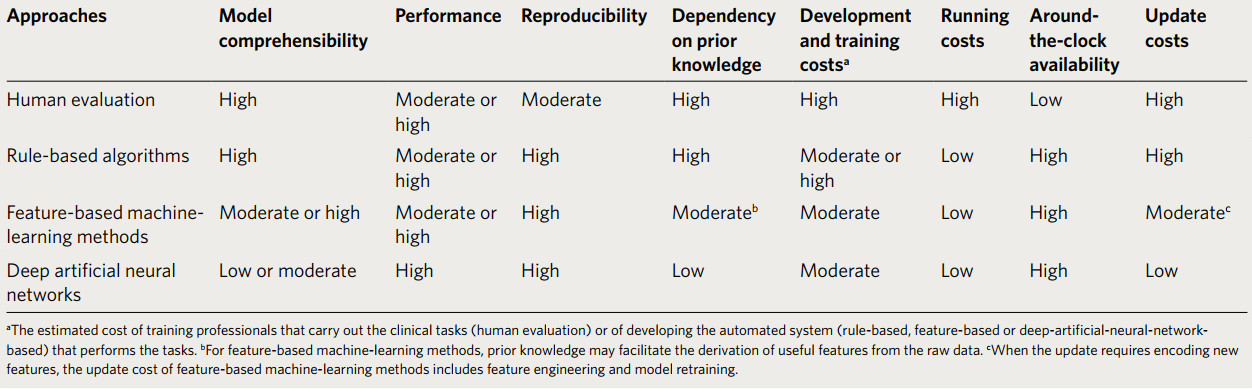
\includegraphics[scale=0.5]{figures/nature.png}
    \caption{Human evaluation vs different types of AI paradigms.}
    \label{fig:Human and AI Approaches}
    \cite{Yu2018}
\end{figure}
\item Naive Bayes Rules 
its name comes from the Bayes theorem on which it is based, applies and calculates conditional probabilities and probabilities. Suitable for large and unknown datasets.
Assumes that features are independent or unrelated between each other. Then the algorithm learns and collects information from each feature class individually.
\end{itemize}
    \item \textbf{Eager} like:
\begin{itemize}
\item Neural Networks
\item SVMs
Intends to maximize the decision boundary margin. The orange dots are the support vector, the points closer to the boundary of decision.

\begin{figure}[ht]
    \centering
    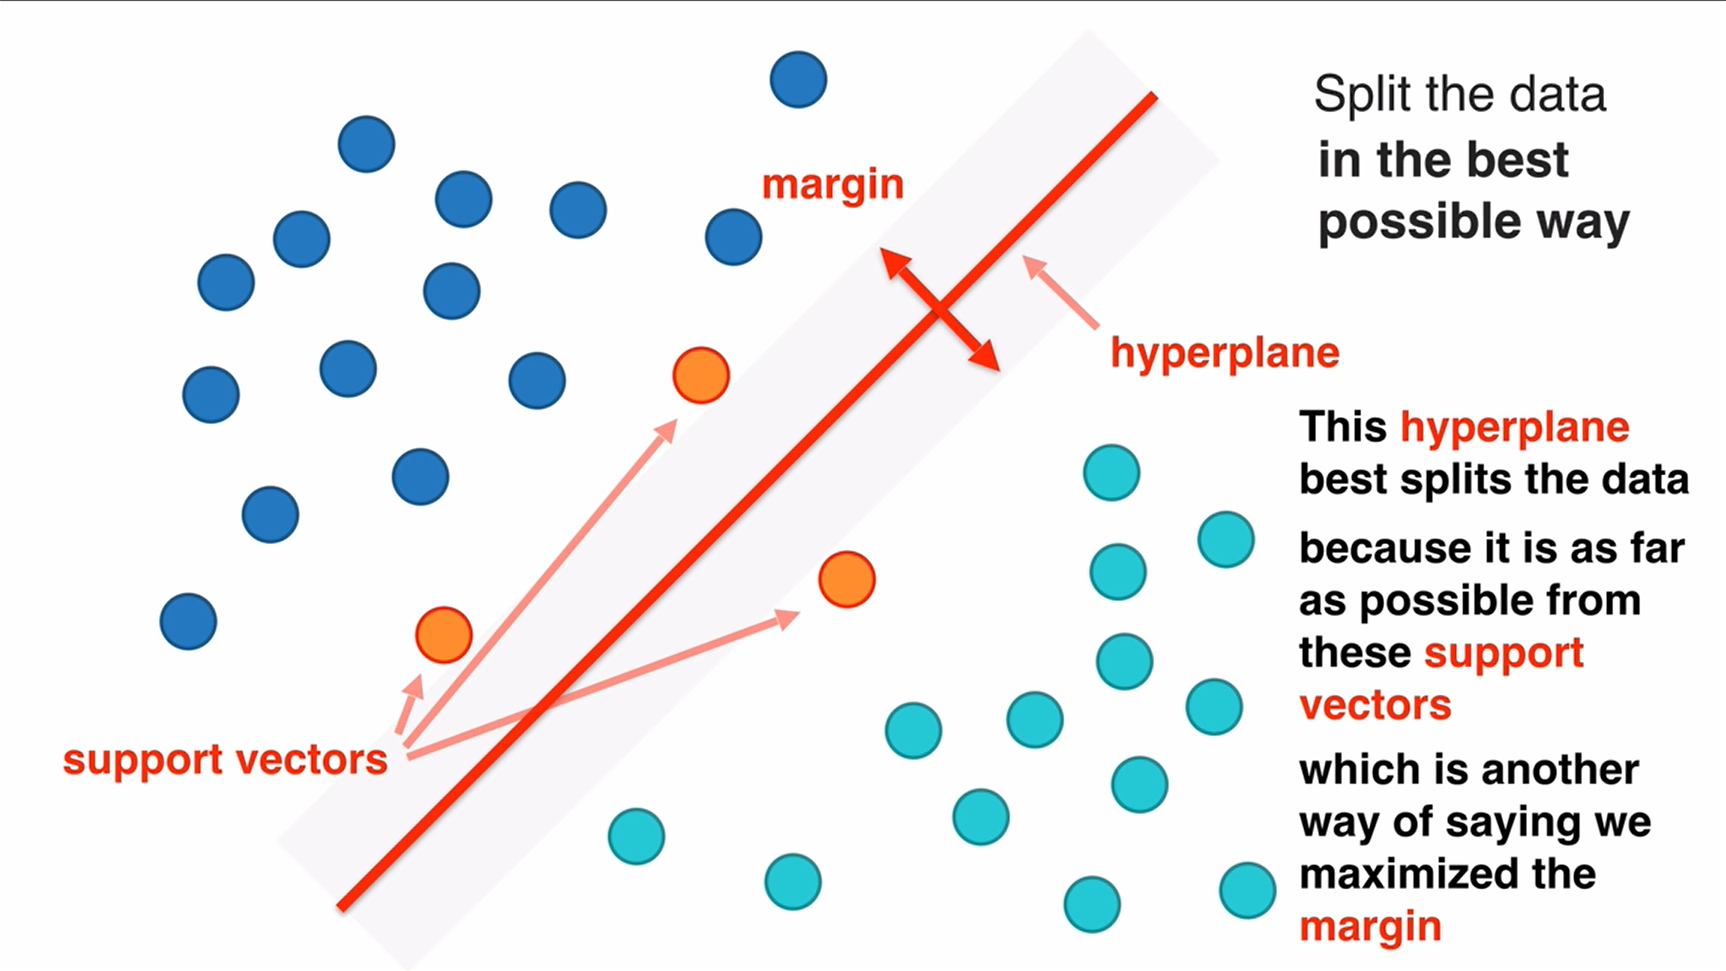
\includegraphics[scale=0.3]{figures/SVM.png}
    \caption{Visual Explanation of SVM}
    \label{fig:SVM}
    \cite{video}
\end{figure}
When the problem is not linearly separable use \textbf{the kernel trick}:
\begin{itemize}
    \item Transition to a higher dimensional space — feature space
    \item Get an optimal boundary
    \item Return to input space
\end{itemize}
\begin{figure}[ht] \centering 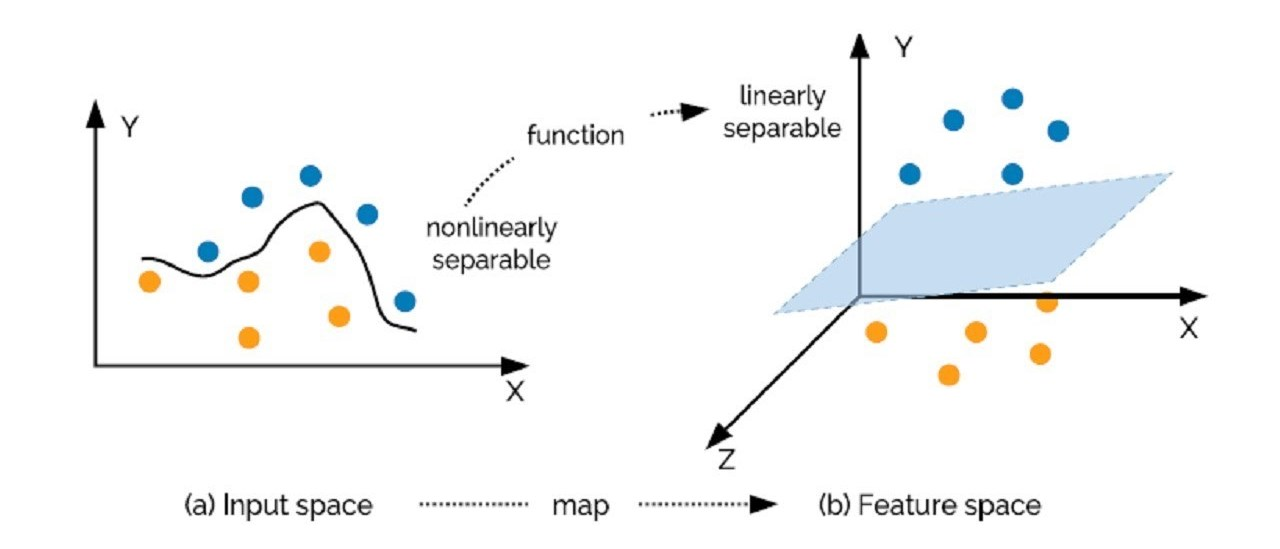
\includegraphics[scale=0.4]{figures/kerneltrick.jpg} \caption{Visual Explanation of the kernel trick} \label{fig:kernelTrick}
\end{figure}



\item Decision trees\\
 
 Hierarchical learning (decomposes in subtrees),
to build one:
\begin{enumerate}
\item Select feature for root node and create a branch for each possible feature value
\item: split instances into subsets: one for each branch extending from the node
\item Repeat for each branch, using only the instances that reach the branch
\end{enumerate}
A selected feature corresponds a question or 
“test” to the database in order to subdivide data until obtaining a branch of the same class called pure leaves.
The goal is to pick the most significant features to subdivide in the faster way possible (minimum number of tests), avoiding overfitting. Note that only 1 feature is picked by the tree if there are more than encodes the same information. The benefits comparing with another algorithms is ease of being understandable by the people, the ability to visualize beyond the algorithms doesn't variant to scaling of the data.
\item Random Forests\\  
Multiple decision trees (ensemble method)  , hierarchical learning, divide and conquer method.
Bootstrapping of samples for each decision tree, and all decision trees, makes a prediction. In regression, makes an average of results. For the other side in classification, makes a soft voting that consist that:
the most probable class, the result of the average of the probabilities of all the probabilities of the predictions of the decision trees, is chosen with the representative label \cite{Muller2017}.
\item Gradient boosted regression trees:
\begin{itemize}
\item used for regression and classification
\item considered one of the most powerful boosting algorithms and widely used on supervised learning, nevertheless, it is required to tune the parameters carefully. 
\item  have a strong pre-pruning which results in shallow trees, typically no more than 5 levels deep consequently is smaller in memory and faster to predict. With more trees and n\texttt{\_}estimators allow more chances to correct mistakes on the training set. 
\item make a serialization of trees with the aim of predicting the error value of the previous tree. And with the learning rate parameter, manage the intensity of correctness in previous trees to the definition in its final result.
\end{itemize}

 \end{itemize}
\end{itemize}

\begin{figure}[ht] \centering 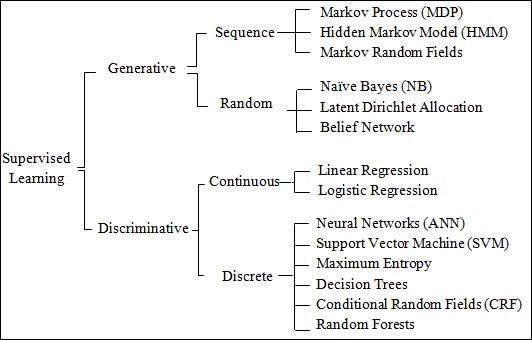
\includegraphics[scale=0.8]{figures/Models representation.jpg}\citet{taxonomy} \caption{Taxonomy of supervised learning algorithms} \label{fig:overviewML} \end{figure}

In this project we focus, use and explore Naive Bayes and a bunch of supervised algorithms of the discriminative and discrete type according to the input data.
\espaco
\espaco
\espaco
\espaco
\espaco
\espaco
\espaco
\espaco
\espaco
\espaco
\espaco
\espaco
\espaco
\espaco
\espaco
\espaco
\espaco
\espaco
\espaco
\espaco
\espaco
\espaco
\espaco
\espaco
\espaco
\espaco
\espaco
\espaco
\espaco
\espaco
\espaco\espaco
\espaco
\espaco
\espaco
\espaco
\espaco
\espaco
\espaco
\espaco
\espaco
\espaco
\espaco
\espaco
\espaco

\espaco

\begin{figure}[ht] \centering 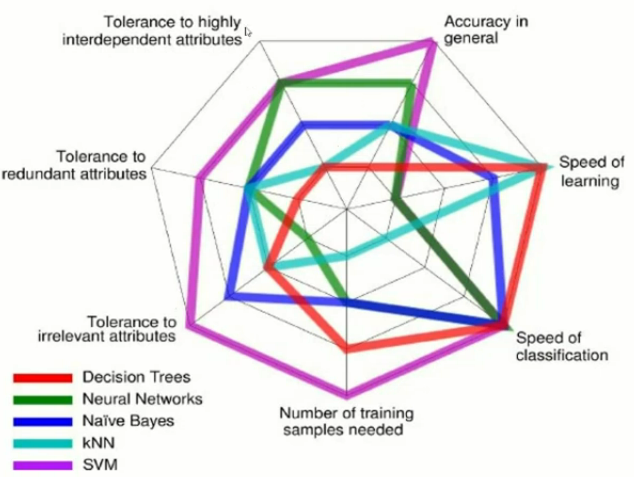
\includegraphics[scale=0.6]{figures/SLalgorithmsCharateristics.png} \caption{Main features of the algorithm } \label{fig:overview} \end{figure}

In this image, we summarize the main features of the algorithms that stand out

\section{Model Evaluation}
\paragraph{} The common practice in the field is to evaluate the model to see if it has the desired performance. 

\section{Pipeline steps of a project}
\begin{itemize}
\item  Collecting the data
\item Get some features
\begin{itemize}
\item  Extract, Analyse and Select
\end{itemize}
\end{itemize}
\begin{itemize}
\item Get a model
\item Train a model
\item Test the model
\item Evaluate the model, adjust and repeat if necessary
\end{itemize}

It is worth pointing out that in case of data limitation, it is important to test with new data. In the evaluation phase, it is expected that:
\begin{itemize}
\item A model is able to generalize from seen data to unseen data.
\item Is “Able” according to some metrics
\end{itemize}

Furthermore, there are statistical methods that allow us to assess the model in terms of predictions and get more information.

\section{Evaluation process}

\begin{itemize}
\item We split the dataset into a training dataset and a test dataset. Under no circumstances, we should use the "test" dataset to train and perform evaluation.
\end{itemize}
 Otherwise, the data will be skewed. That may lead to the misdiagnosis of performance at levels higher than the real ones.
\iffalse
Nevertheless, in some cases like  medicine and biomedical (health in general) areas, there are pre-determined datasets for training and a new dataset(s) for testing.
Typical general use case: Models based on the knowledge of n patients, trying to classify the status of other patients who will arrive.
\fi
Testing the model will take an example from dataset, evaluate it without adjusting the model.
The evaluation result or prediction of the model will be compared with the groundtruth labels.
\begin{itemize}
\item The groundtruth labels are typically not given to the model to make the prediction.
\item They are used to confirm if the prediction was correct or not.
\end{itemize}

Let us examine a simple example with two categorical classes:
"yes" or "no"
If a dataset example has a label "yes" and the model predicted as a "yes", the model as correctly classified the example.
Otherwise, it is an erroneous prediction.

For each input x with groundtruth class y we have:
    Correctly discriminated/classified examples
    Incorrectly discriminated/classified examples
\espaco
\begin{figure}[ht] \centering 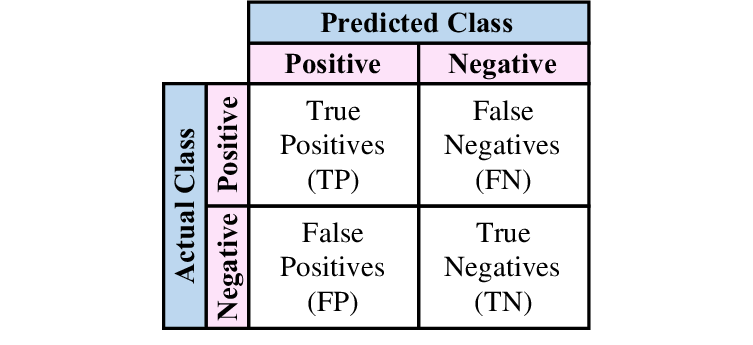
\includegraphics[scale=0.5]{figures/Confusion-matrix.png} 
\caption{Confusion Matrix} \label{fig:confusionM}
\citet{Sheng2020} \end{figure}

From the data in the other table, we can deduce a set of metrics \citet{matrixAi}. 



\begin{figure}[ht] \centering 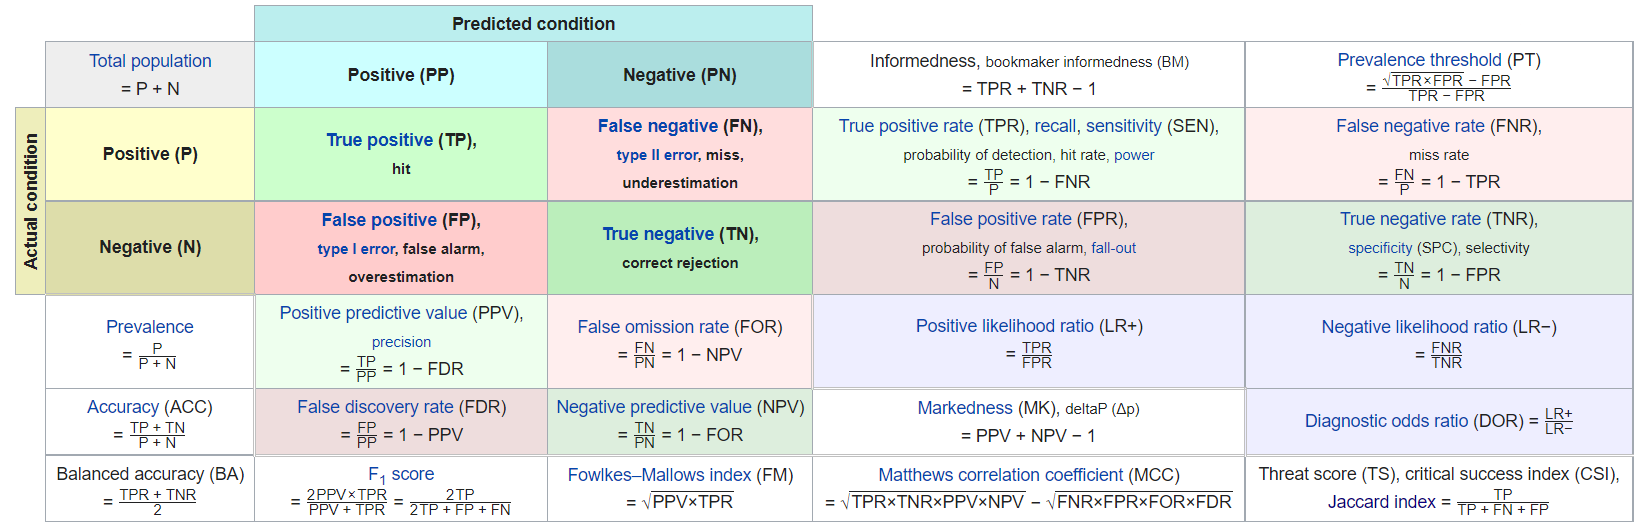
\includegraphics[scale=0.43]{figures/diagram.png} \caption{full matrix confusion table with metrics included}\citet{matrixC}  \label{fig:conf} \end{figure} 

It is good practice to save this data (confusion matrix) because from it, we can calculate everything from these metrics \citet{Powers2011}.




